\documentclass[conference]{IEEEtran}
\IEEEoverridecommandlockouts
\usepackage{cite}
\usepackage{amsmath,amssymb,amsfonts}
\usepackage{algorithmic}
\usepackage{graphicx}
\usepackage{textcomp}
\usepackage{xcolor}
\usepackage{url}
\usepackage{wrapfig}
\usepackage{float}
\usepackage{lscape}
\usepackage{longtable}
\usepackage{booktabs}
\def\BibTeX{{\rm B\kern-.05em{\sc i\kern-.025em b}\kern-.08em
    T\kern-.1667em\lower.7ex\hbox{E}\kern-.125emX}}
\begin{document}

\title{ESCAPE Y2K - An Integrated Escape Room}

\author{Kyle L. Sedgwick, Jake D. Bales, Nami Eskandarian}

\author{\IEEEauthorblockN{1\textsuperscript{st} Kyle L. Sedgwick}
    \IEEEauthorblockA{\textit{College of Engineering} \\
        \textit{University of Utah}\\
        Salt Lake City, U.S \\}
    \and
    \IEEEauthorblockN{2\textsuperscript{nd} Jake D. Bales}
    \IEEEauthorblockA{\textit{College of Engineering} \\
        \textit{University of Utah}\\
        Salt Lake City, U.S \\}
    \and
    \IEEEauthorblockN{3\textsuperscript{rd} Nami Eskandarian}
    \IEEEauthorblockA{\textit{College of Engineering} \\
        \textit{University of Utah}\\
        Salt Lake City, U.S \\}
}



\maketitle

\begin{abstract}
    Escape rooms engage player's critical-thinking skills by placing them inside a locked room
    that requires them to complete puzzles in order to escape. These rooms can be difficult to
    create and control due to the amount of variables present and the fact most of them require
    someone behind the scenes to control the room. “ESCAPE Y2K” is a science fiction analog horror 
    escape room that differs from usual implementations by being completely autonomous. This room 
    uses digital/analog circuit design, image/audio processing, communication protocols, and embedded
    computing for its puzzles and game flow. Players are able to ``travel through time'' to activate
    unique events that assist progression through the room which is controlled by a central server
    that runs a script that sends and receives signals to ESP modules throughout the room. This escape
    room was presented on the Computer Engineering Capstone Demo Day where students and faculty got
    to play with a chance to escape the end of the world!
\end{abstract}

\begin{IEEEkeywords}
    Analog, Embedded Systems, Escape Room, Horror, Interactive, Networking, Science Fiction
\end{IEEEkeywords}

\section{Introduction}
Escape rooms are a fun and engaging way to promote critical thinking and puzzle solving for children and adults
alike. In most established escape rooms, there is a level of behind the scenes interaction with a room operator,
triggering events and unlocking clues as the players progress. This usually works quite well and allows for some
additional variability if the operator is given some creative freedom with how they run the escape room. However,
it also has an inherited limitation with requiring an operator for the room to function. Potential exists for an
autonomous escape room where players follow a game script without the requirement of an external human operator.
This project determines to create a system and design philosophy that allows for a more streamlined and easily modifiable
process for making more complex and dynamic escape rooms. Custom analog and digital systems, as well as a control program
executing on a central server drives the escape room's interactive elements. A solution such as this can greatly
heighten scopes and stakes of escape rooms in the future, providing uniquely exciting experiences for the players
and eases the jobs of the room owners due to automation.
\\
\indent The escape room created for this demonstration is ``ESCAPE Y2K'', a science fiction analog horror experience. 
Inspired by the public panic caused by the Y2K scare, spurred from unknown consequences as digital system
clocks update their year count to '00' and the ambiguity between it's interpretation as '2000' (Y2K) or '1900',
``ESCAPE Y2K'' will be set before the start of the new millennia on January 31, 1999. Due to technological disturbance,
scientists have discovered a creature that will destroy all of humanity, its presence and danger felt in televisions
spread across the room. It is up to the team of players to discover how to send this creature back using puzzle solving
and time travel. Using a remote to forward and reverse a clock that represents in-universe time, they can stop the year
from turning to 2000 which causes total system failure and humanity to end. This inspires the tagline of the game:
``Don't let the clock strike midnight.''

\section{Background}
\indent Escape rooms provide participants with an interactive and exciting puzzle experience.
Players start by being ``locked'' in a room (for safety reasons, players are never really
locked inside) with a set of instructions that lead them through a series of puzzles. Some of
these puzzles are more traditional, such as solving a cypher or figuring out a combination for a lock,
while others make the players think a little bit deeper. Many of these puzzles are on the simple size in
an attempt to have a good balance of fun and difficulty. And, many of these rooms attempt to fit their
puzzles within a certain theme, such as escaping from an Egyptian tomb or trying to escape from the zombie
apocalypse~\cite{wikipediaEscapeRoom}. In order to successfully escape, it is expected that the team of players
all work together to solve every puzzle before time runs out.
\\
\indent Instead of using a large amount of analog puzzles and a ``host'' that is in charge of controlling which parts of
the room are locked and unlocked when players complete certain actions, the room will adapt and progress on its
own as players advance through the various puzzles. A similar idea was done by the 2021 Technical Symposium with
``a course with the overarching goal of designing and constructing an automated escape room''~\cite{germanEscapeRoom}. Outside
of that however, most of the effort will be drawn from a creative process for telling a story; providing presence
to players by immersing them with puzzles using old technology. Old phones, cassette players, televisions, and other
props from the Y2K era will be modified for horror and also allow for puzzle solving. All of this will be done
with the explicit purpose of showing off the wireless communication between the server and the puzzles to keep track
of player progression. 

% ************************************************************************************************************************
% ************************************ THIS IS THE MAIN SECTION TO REVISE FOR THE FINAL REPORT ***************************
% ************************************************************************************************************************
\section{Project Implementation}
While many aspects of our escape room are likely to be somewhat modular, and able to be re-arranged quickly,
some puzzles and in-game events will demand certain elements of the room to be set up in specific locations relative
to each other. For example, the clock controls, game clock, and action clock should all be in close proximity to each
other for ease of access. The CRT TVs should be pointed across the audio cassette player to limit
access during certain events. Finally, props need to be kept in repeatable
locations or lock boxes for consistency in certain puzzles.
\\
\indent In the below diagrams, there are a few key elements to notice. The black boxes with white screens
represent the CRT TVs that have sensors and lights to trigger during in-game events. The
grey towers are filing cabinets, to play into the office aesthetic of the game. The light green slab on the
desks in the corner is where we will have the chessboard, and the yellow head represents one of the busts
that will be included in some puzzles. The center podium will hold the cassette player. Finally, the orange circle
is the time clock, and the nearby green box represents the clock controls.

\subsection{Safe-Cracking Puzzle} % Jake
One of the puzzles that we implemented was a safe cracking puzzle. A hint for this puzzle was recorded on a cassette tape
that would help the players know which numbers they needed to turn the safe to. Once the puzzle was reset by turning the dial
to zero and holding the reset button until the lights flashed, if they turned left until they got to 33, right until they got to 72,
and left again until they reached 11 then the puzzle would be solved! However, players were only able to solve this puzzle when the
player clock (the giant physical clock) displayed a time between 2:15 and 4:30. If all of the above conditions were met, a puzzle box
would open, showing them a plugboard combination.

\subsection{Potentiometer Tuning} % Kyle

The potentiometer puzzle does not provide a direct solution with clear feedback on how it ought to be solved. Instead, 
the four dials need to be placed in the correct orientation by trial and error. This puzzle uses the analog signal inputs 
to find the voltage between each pair of potentiometers for a total of three analog signals. Because this puzzle uses analog 
signals, the ESP module boards are unable to be used as they have no analog capabilities.

\indent The five LEDs on the box light up when the respective voltage across the pair of potentiometers is in the 
correct range (like variable voltage dividers). Because they need to either be determined as ``correct'' or ``incorrect'' 
without any variability between them, the LEDs are set up with digital signals to turn on or off when the correct voltage is 
reached. The first (furthest left) LED turns on when the device has power, and the last (furthest right) only turns on when 
the middle three are illuminated and the correct time frame is shown on the clock. The remaining LEDs are interdependent on one 
another, and do not hint at the correct position of any individual dial, only when all four are in a valid orientation together.


\subsection{Radio Number Station}
The ``number station'' puzzle utilizes the most abstract clue of the three main room puzzles. Unlike the other puzzle clues, 
there is no hint at to what box to use. The tape itself only contains five numbers to align with a box that has five number 
switches. The A side of the tape is played in reverse, so it is nearly impossible to understand what numbers are being stated, 
but a hint printed on a separate sheet of paper urges the player to listen to the message backward by flipping the tape over. 
While this is not how cassette tapes physically work, the B side of the tape is recorded separately with the audio playing 
forward. The static and information on the tape is inspired by “number stations” that were played on radio transmissions during 
the cold war. 

\indent Once the players listen to the recording in the correct orientation, they are able to simply use the number 
switches on the provided box to enter the stated combination. The switches output signals based on the binary values 
of each number, which are decoded by an Arduino Uno to determine when the puzzle is complete. Like the other three initial 
puzzles, it is not fully determined complete until the correct combination is displayed and the correct time frame is reached 
in the game clock.


\subsection{Audio Control and Tapes} % Kyle
The interactive nature of an escape room leads to several factors being included just for the sake of immersion. 
The audio tapes found in the room provide vital hints, but two devices in the room contained additional circuitry 
just to play sound effects without the players controlling them. To accomplish this, we used a ESP module (which 
hijacked the power from the host device boards) and a SD card-read MP3 player (controlled by UART between the ESP and 
itself). The main program would communicate to the ESP modules to play sound effects either randomly, or when particular 
events occur. For example, the ``scream'' sound effect could be played randomly to startle players in the room while the 
``monster footsteps'' would play when the entity was about to trigger its seeking event. For the sake of a more entertaining 
demo, the control panel application could be used to manually play any of the pre-recorded sound effects on the tape player 
or telephone dock.

\indent Recorded audio hints were more vital to the escape room's completion, but did not need to be included in the room's 
programming (with the exception of the final hint). The audio cassettes each contained a hint on the A-side of the 
tape for players to put into the tape player to listen to (which was independent of the remote-triggered sound effects). 
We did not need to modify the mechanical parts of the cassette player for this project, only the electrical parts.

\indent The final hint did require wireless signals to play, as opposed to the recorded tapes. After completing the 
second puzzle, players are given a key that grants them access to a telephone handset. The charging contacts were shorted 
so when they are placed on the dock, the ESP module in the dock detects the phone was put down and signals the internal MP3 
player to play the final hint (which is stored on it's SD card). Unlike the other hints, this recording only plays once, 
demanding the players pay close attention before it turns off for good, adding an additional element of intensity to the room.

\subsection{Adding Time} %Jake

\indent Originally, the idea was to give players a set amount of time to complete the room. Fifteen minutes seemed to be a reasonable amount
time to give them because the puzzles were designed to take about 5 minutes each to solve and there were three puzzles. However,
this all changed when a wonderful idea struck. This idea was motivated by the idea that the players not solving the puzzles might
just be standing around for a large majority of their time in the escape room. This idea came in an effort to keep everyone bustling about, doing
their best to solve the puzzles that had been created for them.
\\
\indent To help remedy this, one puzzle was set aside for a special purpose. This puzzle had a keypad on the face, and when a correct combination was
entered it would give players an extra minute to escape the room. However, in order to make this a bit more complicated, the combinations were broken down
into math problems that, when solved, would reveal one of the combinations. This would help to keep some players busy while others did their best to solve
the room within the alloted time, and also would cause the room to end quicker if players were unable to correctly calculate all ten math equations.

\subsection{TVs, State, and Detection} % Nami

\begin{figure}[ht]
    \centering
    
\includegraphics[width=0.90\columnwidth]{Images/TV_States.png}
    \caption{Screenshots of different videos shown on the TVs. First image is the `Game' state.
    Second image is the `Game' state when it reaches nighttime. Third image is the `Midnight' state. 
    Fourth image is the `Time Travel' state. Fifth image is the `Seek' state. Sixth image is the `Monster' state.}
    \label{fig:tv}
\end{figure}

\indent In accordance with the time period the game is set in, a CRT TV and monitor were procured and used to capture the state of the game
as players make their way through the escape room. A mini PC is connected to each TV and using python-vlc, a library that links VLC Media Player
and Python, the mini PC receives signals from the server to play certain videos. Figure~\ref{fig:tv} provides screenshots of these different states
which play on the TVs with audio playing through bluetooth speakers located on the edges of the room for surround sound. A game timer is also shown
on each TV to show exactly how much real-life time players have left to complete the room.

\begin{figure}[ht]
    \centering
    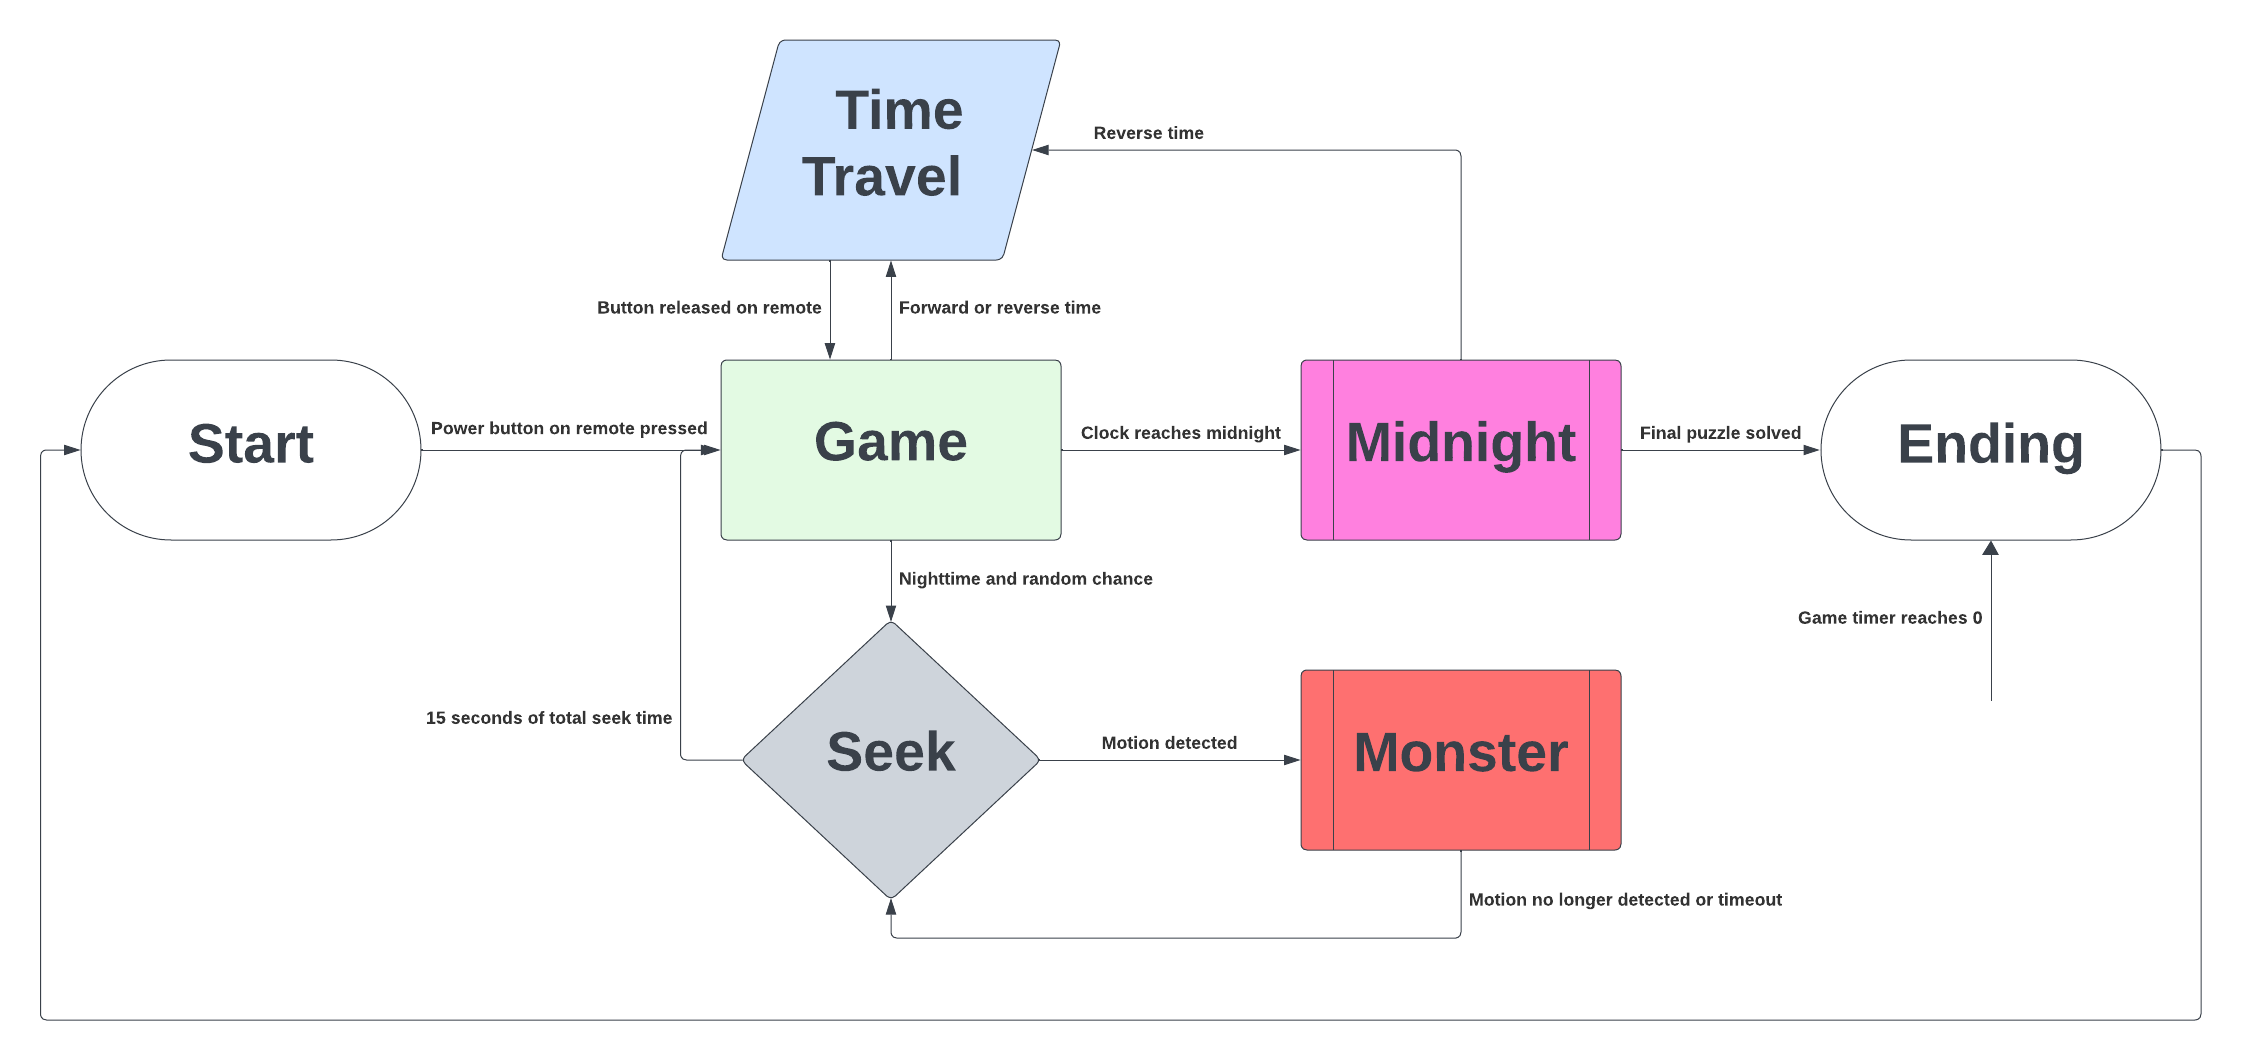
\includegraphics[width=0.90\columnwidth]{Images/state_flow.png}
    \caption{A flowchart representing the different states of the game.}
    \label{fig:pir}
\end{figure}

\subsubsection{Start}

\indent This is the resting state of the game where nothing is happening and is simply waiting for players to start. All TVs will be dark during this state.
When the players wish to play the game, they push the power button on the remote and point it at the TV to start the clock, game timer, and move to the `Game' state.

\subsubsection{Game}

\indent This is the general state of the game. An animated Windows XP Wallpaper with serene ambience will play with the time of the clock being reflected by the video.
Every ten ticks of the clock, the mini PC will receive a signal to update the time of the video for any syncing issues. When the clock reaches 60 ticks,
the color of the video will distort and the ambience will turn into a darker, more horrifying sound. This is to represent that the players are getting
closer to midnight, and will also act as a signal that the monster is able to seek for the players.

\subsubsection{Midnight (Panic State)}

\indent The `Midnight' state is considered a panic state that will deplete the game timer at a quicker pace than usual. This state is reached when
the clock has reached 12:00 and will only stop when the clock is reversed or the game ends. The Windows XP wallpaper has gone fully distorted with
a bell tolling the new millenium has reached and distorted screaming of the end of the world. It's unadvised players let the game get to this state
since they will incur time penalties, however this state is required to solve the final puzzle as a way to introduce tension as the room gets to a close.

\subsubsection{Time Travel}

\indent When the players use the remote to either forward or reverse the clock, the screen will resemble fast forwarding or reversing an old VHS. When
the game is at this state, the monster cannot show up.

\begin{figure}[ht]
    \centering
    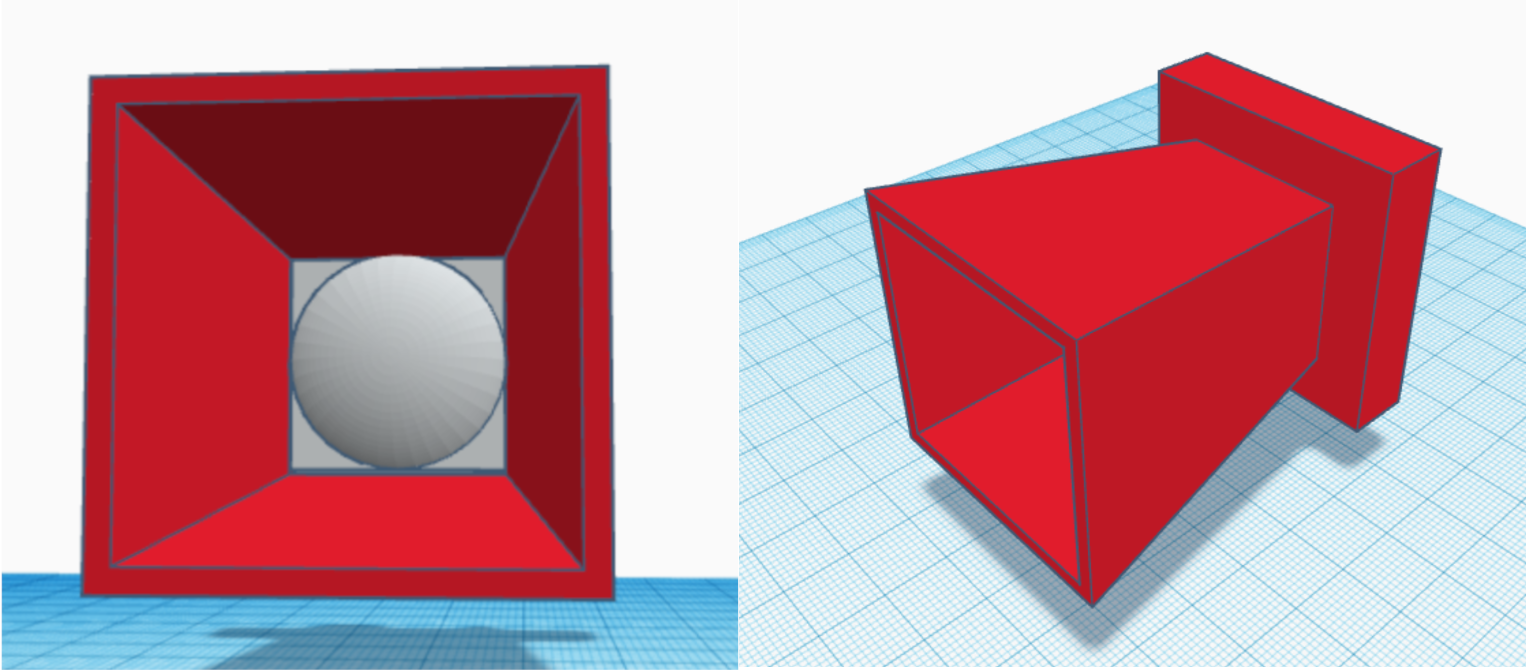
\includegraphics[width=0.90\columnwidth]{Images/PIR.png}
    \caption{CAD screenshots of the print used for the PIR motion detectors located on top of the TVs.
    The motion detector is inserted in the bottom facing into it, with its range limited by the cone shape of the print.}
    \label{fig:pir}
\end{figure}

\subsubsection{Seek}

\indent When the clock is considered to be at ``nighttime'' (which is represented by the usual game video being reddish) then the monster will search
the room for the players on random chance. A PIR motion sensor was used to detect motion and located on top of each TV with a print as shown in Figure ~\ref{fig:pir} to restrict its searching area to
act as the TVs field of vision. To warn players of this state, the cassette player will play a sound of looming footsteps before the eye appears on
the screen searching around the room. This will last for 15 seconds as the motion sensor now starts polling to see if motion is detected. When motion is
detected, the state will change to the `Monster' state until motion is no longer detected, in which it returns to this tate to finish the 15 seconds it
searches for. When the 15 seconds are up, it will return to the `Game' state. The clock is paused during this state.


\subsubsection{Monster (Panic State)}

\indent The `Monster' state is considered a panic state that will deplete the game timer at a quicker pace than usual. This state is reached when motion
is detected during the `Seek' state and will revert to the `Seek' state when motion is no longer detected. There is also a timeout of 5 seconds in case
hardware issues arise to not crushingly punish the players. During this state, the monsters presence will be felt in the room as a scream and 
horrible noises are played to induce stress in the players. This is a horror experience, after all. 

\subsubsection{Ending}

\indent There are two endings to the escape room on a win and a loss. When the game timer reaches 0, a video will play ``ejecting'' a VHS before static
fills the screen. When the players solve the final puzzle, everything will shut down and remain dark for a few seconds before a video will play showing old
footage of old new years celebration for the year 2000. These videos cut to black at the end of them, signifying the end of the escape room. The players can
then be either proud of their win or lament their loss depending on which ending they got. 

\subsection{Time Control and the Clock} % Kyle

\subsection{Wireless Communication and Circuit Design} %Jake
One of the central ideas behind what makes this escape room different from other escape rooms is that all of the puzzles are able to communicate
wirelessly with a central server, indicating when they had been solved. Using this information, the server could then communcate wirelessly with
the locked puzzle boxes, telling them to open without needing any external intervention. This paradigm was used extensively throught the escape
room, allowing special events to trigger themselves and allowing certain components to connect and function synchronously, giving the room a 
sense of interconnectedness. This wireless communication was achieved through the use of a dummy WiFi router and arduinos with ESP modules
attached to them, restricting their connection to the internet as a whole but allowing them to talk on an interconnected LAN network.
\\
\indent This network was further enhanced by the implementation of a server, which would propagate signals to any module that may need to be informed
of an event and keep track of the current state of the room. An "admin control panel" was also developed, which allows any user that is "behind the
scenes" to activate special events, lock or unlock boxes, and reset the current state of the room.



\begin{figure}[ht]
    \centering
    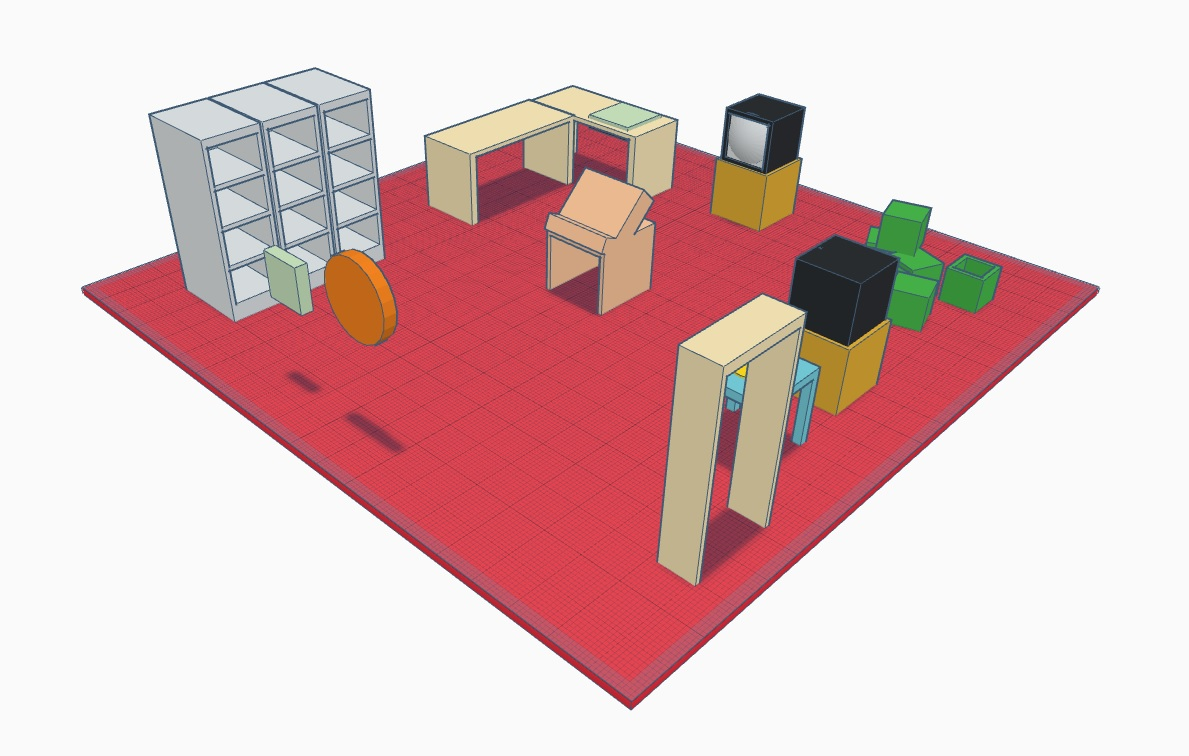
\includegraphics[width=0.90\columnwidth]{Images/EscapeRoomIsoFront.jpg}
    \caption{Front isometric scale depiction of the initial escape room layout.}
\end{figure}

\begin{figure}[ht]
    \centering
    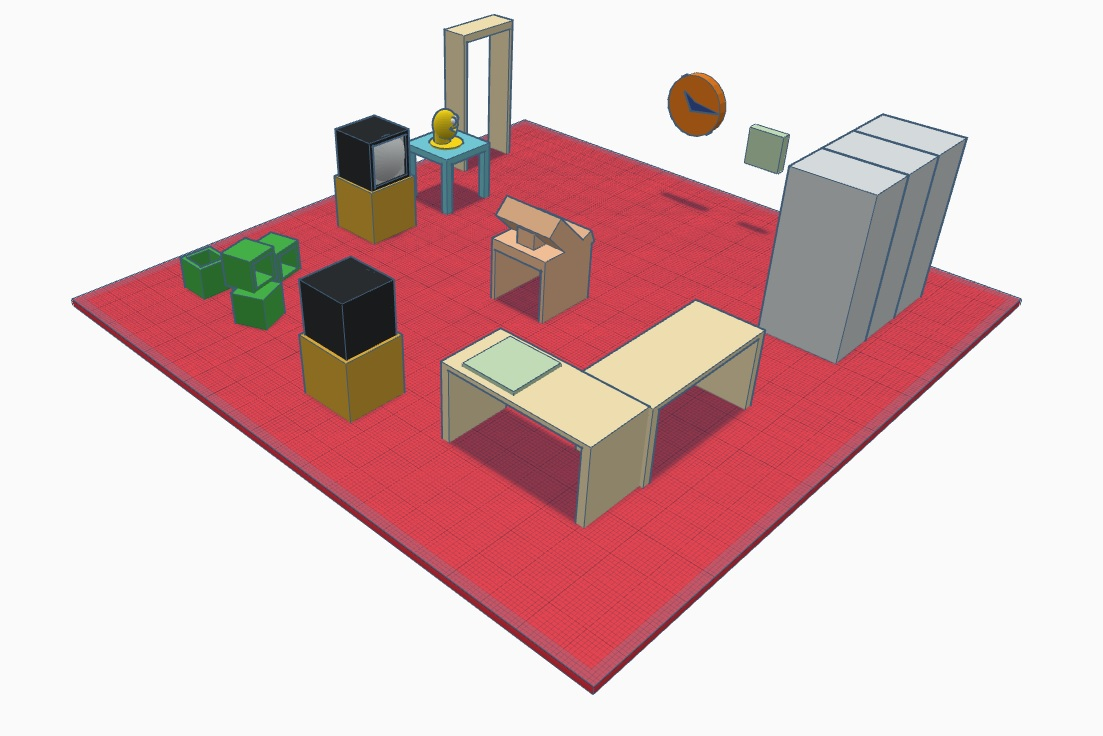
\includegraphics[width=0.75\columnwidth]{Images/EscapeRoomIsoRear.jpg}
    \caption{Rear isometric scale depiction of the initial escape room layout.}
\end{figure}

% *************************************************************************************************************************************
% ************************************* THIS SECTION MUST BE REVISED ******************************************************************
% *************************************************************************************************************************************
\section{Evaluation} % Kyle
``ESCAPE Y2K'' was completed, and fully functional as a computer controlled escape room experience. For demo day itself, 
the control panel for the room was used to provide assistance and allow other guests to play sound effects remotely to 
interact with the room if they could not participate actively. While the technical aspects of Escape Y2K were all 
implemented and functional for the demonstration, there were a few aspects that could be improved for later revisions 
of this, or other, computer controlled escape rooms.

\subsection{Functionality}
There were several physical aspects of ``ESCAPE Y2K'' that could have failed during the demonstration, from dislodged wires, 
misaligned clock hands for the slot-interrupt sensors, jammed autoboxes, or general hardware failure. Thankfully, due 
to careful consideration of transportation and attention during re-assembly, these were all successfully avoided. If 
additional funding were available, it would be possible to make printed circuit boards for all breadboard components, 
which are the biggest concern for re-assembly and reliability issues.

\indent After the approximate hour and 45 minutes of re-assembly, the room was able to be fully tested for function 
and connectivity reliability before guests were let into the room. While being used, none of the above concerns caused 
any practical issue for guests, but unfortunately, no teams managed to finish the escape room due to time constraints 
(which will be addressed in the following subsections). While everything physically operated as it should, there were a 
few aspects that a second revision would address to make things run even smoother.

\subsection{Mechanical Shortcomings}
Many components of student made projects can be extremely fragile due to limitations of time, funding, or uncontrollable 
factors like mistakes on the side of the end-user. Thankfully, the users did not cause any problems over the duration of 
the demonstration, and nothing had serious reliability issues. However, there are a few aspects that had potential to cause 
issues if factors were slightly different.

\indent One such concern is the fragility of puzzle boxes and the clock. Because the clock relies on a relatively cheap 
stepper motor, custom 3D printed mounts, and finicky slot-interrupters, there are multiple aspects that hold potential 
of breaking. Should the clock module be revised, we would 3D print a full enclosure for the motor that could house the 
separate encoder much closer. By covering the motor entirely, it would prevent accidental dislodging or mechanical 
movement not detected by the encoder. The slot interrupters could have a metal wing affixed below the clock hand, to be 
more stable and secure than the tape wing used for the first revision. 

\indent Concerns on the fragility of puzzles could simply be solved by making custom PCBs would remove reliability concerns 
of loose wiring. With additional funding, the containers could also be made from more rugged materials, rather than 3D 
printed (although 3D printing was find for demonstration purposes).

\subsection{Creative Adjustments}
Guests of the room provided feedback from their experiences to improve a revised escape room. Much of this feedback was 
not necessarily on the technical side, but rather for the experiential aspects of the room, such as immersion and logical 
flow. For individuals inexperienced with escape rooms, having a system that does not require an operator can make it extremely 
difficult to try to understand where to start looking in the room, so some changes can benefit less experienced players.

\indent The biggest and most consistent piece of feedback received was on timing. Eight minutes is simply not enough time to 
get situated in the room and rationally look for clues. Our basic attempt at improving this was the ability to add time back 
with the use of codes. However, with such a short initial time, this still was not particularly helpful. The unique ability 
to get working time back is central to ``ESCAPE Y2K'', so the code system could be made more accessible to allow for more time 
extensions. The easiest (and realistically intended) solution is to give players more base time when the room starts. With the 
amount and complexity of puzzles, 20 minutes would be an ideal starting time for the room.

\indent Another unique aspect of ``ESCAPE Y2K'' that could use play-tuning is the appearance of the entity through the television 
monitors. While its presence was restricted to about a one-percent chance of appearing every second while the clock was after 
8:00 PM, these chances could stack on with additional time if the chance was completed while the entity was already seeking in 
the room. Simply preventing this from happening could let players be less intruded by the entity, while still keeping it as an 
important aspect of the room. As this is purely a creative change, it's ideal implementation would still need to be flexible to 
further feedback as changes are continually made.


\section{Conclusion} % Nami

\indent One of the greatest joys of creation is to allow others to experience your creation for the first time. This prototype
for a completely autonomous escape room had one of the underappreciated pleasures of allowing the ability to simply watch players play the room.
This gave us lots of time to take notes on what worked and what was difficult without worrying about control, but it also exhibited
the spark of ideas and creative problem solving that makes escape rooms so captivating. Setting puzzles up to communicate with each other
wirelessly presented opportunities for complex interactions with players alongside maintaining their progress. With further development, more and more
escape rooms can utilize smart engineering for rooms that run by themselves (with supervision for safety in case of failure). This could also open up
even more opportunities for increasingly complex game mechanics alongside standard puzzle solving which can release the floodgates for advanced experiences. 
Ideas include a random selection of puzzles each playthrough, passcodes that keep changing, hacking into computers, keys using RF reading, and many more.
Like how ``ESCAPE Y2K'' ends with the new millennia, this concept could also usher in a new age in 
escape rooms that redefine what it takes to escape.

\section{Appendix A: Reference Material}

\subsection{Bill of Materials}
In order to have a functioning project that we can be proud of, we are going to need a lot of materials.
A list of these materials have been included below
\begin{itemize}
    \item Programmable microcontrollers
    \item Analog clock
    \item Cameras
    \item Small CRT televisions
    \item Audio cassette player
    \item Writable audio cassette tapes
    \item MP3 digital audio controller
    \item Speakers
    \item Motors (To act as lock releases)
    \item Solenoids
    \item LED Display
    \item Adjustable RGB lights
    \item Wireless communication modules
    \item Storage containers
    \item Busts with detachable modules
\end{itemize}

\section{Appendix B: Troubles of note during development}

\begin{thebibliography}{00}

    \bibitem{wikipediaEscapeRoom} “Escape room,” Wikipedia, 10-Feb-2023. [Online]. Available: \url{https://en.wikipedia.org/wiki/Escape_room}. [Accessed: 24-Mar-2023].
    \bibitem{germanEscapeRoom} M. Pfeifer, B. Völker, S. Böttcher, S. Köhler, and P. M. Scholl, “Teaching embedded systems by constructing an escape room,” Proceedings of the 52nd ACM Technical Symposium on Computer Science Education, 2021.    
    \bibitem{whatIsAnEscapeRoom} A. Ascalon, “Escape rooms: Everything you need to know (2022),” Escape Rooms | Everything You Need To Know (2022), 01-Dec-2022. [Online]. Available:  \url{https://theescapegame.com/blog/what-is-an-escape-room/}. [Accessed: 24-Mar-2023].
    \bibitem{wifiVsZigbee} B. Priya, “What are the differences between Zigbee and Wi-Fi,” Tutorials Point, 17-Mar-2022. [Online]. Available: \url{https://www.tutorialspoint.com/what-are-the-differences-between-zigbee-and-wi-fi}. [Accessed: 03-May-2023].

\end{thebibliography}




\end{document}
